\documentclass[class=article,10pt,crop=false]{standalone}
\usepackage{standalone}
\usepackage{preamble}

\begin{document}
\begin{multicols}{2}[\section{Algebraic structures}]
\subsection{Groups}
\subsubsection*{Groups and subgroups}
\begin{definition}[Group]
A group is a non-empty set $G$ together with a binary operation \begin{align*}
    \cdot:G\times G&\longrightarrow G\\
    (g_1,g_2)&\longmapsto g_1\cdot g_2
\end{align*}
satisfying the following properties:
\begin{enumerate}
    \item Associativity: $$(g_1\cdot g_2)\cdot g_3=g_1\cdot(g_2\cdot g_3)\quad\forall g_1,g_2,g_3\in G.$$
    \item Identity element: $$\exists e\in G:e\cdot g=g\cdot e=g\quad\forall g\in G\footnote{From now on, we will denote $e$ or $e_G$ the identity element of the group $(G,\cdot)$.}.$$
    \item Inverse element: $$\forall g\in G, \exists h\in G:g\cdot h=h\cdot g=e.$$ We denote $h$ by $g^{-1}$.
\end{enumerate}
If, moreover, we have $g_1\cdot g_2=g_2\cdot g_1$ $\forall g_1,g_2\in G$, we say the group $(G,\cdot)$ is \textit{commutative} or \textit{abelian}\footnote{Sometimes to simplify the notation and if the context is clear, we will refer to $G$ directly as the group as well as the set.}.
\end{definition}
\begin{lemma}
Let $(G,\cdot)$ be a group. Then,
\begin{enumerate}
    \item The identity element is unique.
    \item Given an element $g\in G$, $\exists! h\in G$ such that $g\cdot h=h\cdot g=e$.
    \item Given $g,h\in G$ such that $g\cdot h=e$, we have $h=g^{-1}$.
\end{enumerate}
\end{lemma}
\begin{definition}[Subgroup]
Let $(G,\cdot)$ be a group and $H$ be a subset of $G$. $(H,\cdot)$ is called a \textit{subgroup} of $(G,\cdot)$\footnote{Sometimes we will denote that $(H,\cdot)$ is a subgroup of $(G,\cdot)$ as $H\leq G$.} if satisfies:
\begin{enumerate}
    \item If $h_1,h_2\in H$, then $h_1\cdot h_2\in H$.
    \item $e\in H$.
    \item If $h\in H$, then $h^{-1}\in H$.
\end{enumerate}
\end{definition}
\begin{prop}
Let $(G,\cdot)$ be a group and $H\ne\emptyset$ be a subset of $G$. Then $$(H,\cdot)\text{ is a subgroup}\iff h_1\cdot h_2^{-1}\in H\quad\forall h_1,h_2\in H.$$
\end{prop}
\begin{prop}
If $(H,+)$ is a subgroup of $(\mathbb{Z},+)$, then $\exists n\in\mathbb{Z}$ such that $H=n\mathbb{Z}=\{nk:k\in\mathbb{Z}\}$.
\end{prop}
\begin{prop}
Let $(G_i,*_i)$, for $i=1,\ldots, n$, be groups. Then the product $$(G_1,*_1)\times\cdots\times(G_n,*_n)$$ induces a group with the operation $\cdot$ defined as $$(g_1,\ldots,g_n)\cdot(g_1',\ldots,g_n')=(g_1*_1g_1',\ldots,g_n*_ng_n'),$$ where $g_i,g_i'\in G_i$.
\end{prop}
\begin{definition}
The \textit{order of a group $(G,\cdot)$} is the number of elements in its set, that is, $|G|$.
\end{definition}
\begin{lemma}
Let $(G,\cdot)$ be a group and $\{(H_i,\cdot):i\in I\}$ a set of subgroups of $(G,\cdot)$. Then if $$H=\displaystyle\bigcap_{i\in I}H_i,$$ we have that $(H,\cdot)$ is also a subgroup of $(G,\cdot)$.
\end{lemma}
\begin{definition}
Let $(G,\cdot)$ be a group and $X\subseteq G$ a subset of $G$. The \textit{subgroup of $(G,\cdot)$ generated by $X$}, $(\langle X\rangle,\cdot)$, is the smallest subgroup of $(G,\cdot)$ containing $X$, that is, $$\langle X\rangle=\bigcap_{X\subseteq H\leq G}H.$$
\end{definition}
\begin{definition}
Let $(G,*)$ be a group, $g\in G$ and $n\in\mathbb{Z}$. We define $g^n$ as: $$g^n=\left\{\begin{array}{lll}
    g*\overset{(n)}{\cdots}* g & \text{if} & n>0  \\
    1 & \text{if} & n=0  \\
    (g^{-1})*\overset{(|n|)}{\cdots}*(g^{-1}) & \text{if} & n<0 
\end{array}\right.$$
\end{definition}
\begin{lemma}
Let $(G,\cdot)$ be a group and $g\in G$. Then for all $n,m\in\mathbb{Z}$ we have
\begin{enumerate}
    \item $g^n\cdot g^m=g^{n+m}=g^m\cdot g^n$.
    \item $(g^n)^m=g^{nm}=(g^m)^n$.
\end{enumerate}
\end{lemma}
\begin{definition}
Let $(G,\cdot)$ be a group and $g\in G$. A subgroup $(\langle g\rangle,\cdot)$ of $(G,\cdot)$ generated by a single element $g$ is called a \textit{cyclic group}.
\end{definition}
\begin{prop}
Let $(G,\cdot)$ be a group and $g\in G$. Then, $$\langle g\rangle=\bigcup_{i\in\mathbb{Z}}\{g^i\}.$$
\end{prop}
\begin{definition}
Let $(G,\cdot)$ be a group and $g\in G$. The \textit{order of $g$} is $o(g):=|\langle g\rangle|$.
\end{definition}
\begin{prop}
Let $(G,\cdot)$ be a group and $g\in G$. Then, $$o(g)=\min\{i\in\mathbb{N}:g^i=e\}.$$ If no such $i$ exists, we say $o(g)=\infty$.
\end{prop}
\begin{corollary}
Let $n\in\mathbb{N}$, $n>1$, and $\Bar{a}\in\mathbb{Z}/n\mathbb{Z}$. Then: $$o(\Bar{a})=\frac{n}{\gcd(a,n)}.$$
\end{corollary}
\begin{lemma}
Let $(G,\cdot)$ be a group, $g\in G$ and $o(g)=n$. Then:
\begin{enumerate}
    \item $g^m=e\iff n\mid m$.
    \item $g^m=g^{m'}\iff m=m'\mod{n}$.
    \item If $0\leq i\leq n$, then $g^{-i}=(g^i)^{-1}=g^{n-i}$.
\end{enumerate}
\end{lemma}
\begin{corollary}
Let $(G_i,*_i)$, for $i=1,\ldots, n$, be groups. For $i=1,\ldots,n$, let $g_i\in G_i$ and consider the element $g=(g_1,\ldots,g_n)\in(G_1,*_1)\times\cdots\times(G_n,*_n)$. Then: $$o(g)=\lcm(o(g_1),\ldots,o(g_n)).$$
\end{corollary}
\begin{prop}
Let $(G,*)$ be a group and $X\subseteq G$ be a subset of $G$. Then: $$\langle X\rangle=\{e\}\cup\{g_1^{\alpha_1}*\cdots* g_n^{\alpha_n}:n\in\mathbb{N},\alpha_i\in\mathbb{Z},g_i\in X\}.$$
\end{prop}
\subsubsection*{Group morphisms}
\begin{definition}[Group morphism]
Let $(G,*)$, $(H,\cdot)$ be two groups. A \textit{morphism from $(G,*)$ to $(H,\cdot)$} is a function $\phi:G\rightarrow H$ such that $$\phi(g_1*g_2)=\phi(g_1)\cdot\phi(g_2)\quad\forall g_1,g_2\in G.$$
\end{definition}
\begin{lemma}
Let $\phi:G_1\rightarrow G_2$ be a morphism between $(G_1,*)$ and $(G_2,\cdot)$. Then,
\begin{enumerate}
    \item $\phi(e_1)=e_2$.
    \item $\phi(g^{-1})=\phi(g)^{-1}\quad\forall g\in G_1$.
    \item $\phi(g^n)=\phi(g)^n\quad\forall g\in G_1$ and $\forall n\in\mathbb{Z}$.
\end{enumerate}
\end{lemma}
\begin{definition}
We say a subgroup $(H,\cdot)$ of a group $(G,\cdot)$ is \textit{normal}, $H\lhd G$, if and only if $\forall h\in H$ and $\forall g\in G$, we have $g\cdot h\cdot g^{-1}\in H$.
\end{definition}
\begin{definition}
Let $(G_1,*)$, $(G_2,\cdot)$ be two groups and $\phi:G_1\rightarrow G_2$ be a group morphism. The \textit{kernel of $\phi$} is $$\ker\phi=\{g\in G_1:\phi(g)=e_2\}.$$ The \textit{image of $\phi$} is $$\im\phi=\{h\in G_2:\phi(g)=h\text{ for some }g\in G_1\}.$$
\end{definition}
\begin{prop}
Let $(G_1,*)$, $(G_2,\cdot)$ be two groups and $\phi:G_1\rightarrow G_2$ be a group morphism. Then:
\begin{enumerate}
    \item $(\ker\phi,*)$ is a normal subgroup of $(G_1,*)$ and $(\im\phi,\cdot)$ is a subgroup of $(G_2,\cdot)$.
    \item Let $g,g'\in G_1$. The following statements are equivalent:
    \begin{enumerate}
        \item $\phi(g)=\phi(g')$.
        \item $g*g'^{-1}\in\ker\phi$.
        \item $g'^{-1}*g\in\ker\phi$.
    \end{enumerate}
    \item $\phi$ is injective if and only if $\ker\phi=\{e_1\}$.
    \item $\phi$ is surjective if and only if $\im\phi=G_2$.
\end{enumerate}
\end{prop}
\begin{definition}
Let $(G,*)$, $(H,\cdot)$ be two groups. An \textit{isomorphism between $(G,*)$ and $(H,\cdot)$} is a bijective morphism between $(G,*)$ and $(H,\cdot)$.
\end{definition}
\begin{prop}
Let $(G_1,\cdot_1)$, $(G_2,\cdot_2)$, $(G_3,\cdot_3)$ be three groups and $\phi:G_1\rightarrow G_2$, $\psi:G_2\rightarrow G_3$ be two group morphisms. Then the composition $\psi\circ\phi$ is also a group morphism.
\end{prop}
\begin{prop}
Let $(G_1,*)$, $(G_2,\cdot)$ be groups and let $\phi: G_1\rightarrow G_2$ be an isomorphism. Then $\phi^{-1}: G_2\rightarrow G_1$ is also an isomorphism.
\end{prop}
\begin{definition}
Two groups $(G_1,*)$, $(G_2,\cdot)$ are \textit{isomorphic}, $G_1\cong G_2$, if there exists an isomorphism $\phi:G_1\rightarrow G_2$.
\end{definition}
\begin{theorem}[Classification of cyclic groups]
Let $(G,\cdot)$ be a group and $g\in G$ be an element such that $\langle g\rangle=G$.
\begin{itemize}
    \item If $|G|=\infty$, then $G\cong\mathbb{Z}$. We can define the isomorphism as follows: 
    \begin{align*}
        \phi:\mathbb{Z}&\longrightarrow G\\
        k&\longmapsto g^k
    \end{align*}
    \item If $|G|=n$, then $G\cong\mathbb{Z}/n\mathbb{Z}$. We can define the isomorphism as follows: 
    \begin{align*}
        \phi:\mathbb{Z}/n\mathbb{Z}&\longrightarrow G\\
        \Bar{k}&\longmapsto g^k
    \end{align*}
\end{itemize}
\end{theorem}
\begin{corollary}
Let $(G,\cdot)$ be a group and $g\in G$ be such that $\langle g\rangle=G$. Then all subgroups of $G$ are cyclic. Moreover:
\begin{itemize}
    \item If $|G|=\infty$, subgroups of $(G,\cdot)$ are of the form $\langle g^n\rangle$, $n\in\mathbb{N}\cup\{0\}$. 
    \item If $|G|=n$, then there is a unique subgroup $(H,\cdot)$ of $(G,\cdot)$ for every divisor $d>0$ of $n$. In fact, if $n=dq$, then $H=\langle g^q\rangle$ and $|H|=d$.
\end{itemize}
\end{corollary}
\begin{definition}
Let $X$ be a set. We define the \textit{symmetric group $(S(X),\circ)$}, where $$S(X)=\{f:X\rightarrow X:f\text{ is bijective}\}\footnote{Observe that if $X=\{1,\ldots,n\}$, then $S(X)=S_n$.}.$$ 
\end{definition}
\begin{definition}
Let $(G,\cdot)$ be a group. We define the functions
\begin{align*}
    \ell_g:G&\longrightarrow G&r_g:G&\longrightarrow G\\
    x&\longmapsto g\cdot x &x&\longmapsto x\cdot g
\end{align*}
\end{definition}
\begin{lemma}
Let $(G,\cdot)$ be a group. The functions $\ell_g$, $r_g$ are bijective and its inverses are $\ell_{g^{-1}}$, $r_{g^{-1}}$, respectively.
\end{lemma}
\begin{prop}
Let $(G,\cdot)$ be a group. We define the functions:
\begin{align*}
    \phi:G&\longrightarrow S(G)&\psi:G&\longrightarrow G\\
    g&\longmapsto \ell_g &g&\longmapsto r_{g^{-1}}
\end{align*}
Then, $\phi$ and $\psi$ are injective group morphisms.
\end{prop}
\begin{theorem}[Cayley's theorem]
Let $(G,\cdot)$ be a group. Then there is an injective morphism $$\phi:G\longrightarrow S(G)$$
\end{theorem}
\begin{corollary}
If $(G,\cdot)$ is a group with $|G|=n$, we can think $(G,\cdot)$ as a subgroup of $(S_n,\circ)$.
\end{corollary}
\subsubsection*{Cosets}
\begin{definition}\label{AS_equiv} 
Let $(G,\cdot)$ be a finite group, $(H,\cdot)$ be a subgroup of $(G,\cdot)$ and $g_1,g_2\in G$. 
\begin{itemize}
    \item We say $g_1\sim g_2\iff g_1\cdot g_2^{-1}\in H$.
    \item We say $g_1\approx g_2\iff g_2^{-1}\cdot g_1\in H$.
\end{itemize}
\end{definition}
\begin{lemma}
Let $(G,\cdot)$ be a finite group and $(H,\cdot)$ be a subgroup of $(G,\cdot)$. Then:
\begin{enumerate}
    \item $\sim$ and $\approx$ are equivalence relations.
    \item If $g\in G$, then 
    \begin{gather*}
        [g]_\sim=H\cdot g=\{h\cdot g:h\in H\},\\ [g]_\approx=g\cdot H=\{g\cdot h':h'\in H\}.
    \end{gather*}
    Usually we say that $H\cdot g$ are the \textit{right cosets in $G$} and $g\cdot H$, the \textit{left cosets in $G$}. 
\end{enumerate}
\end{lemma}
\begin{definition}
Let $(G,\cdot)$ be a finite group and $(H,\cdot)$ be a subgroup of $(G,\cdot)$. We define the \textit{set of left cosets} and the \textit{set of right cosets} as follows:
$$\quot{G}{\sim}=\{H\cdot g:g\in G\},\quad\quot{G}{\approx}=\{g\cdot H:g\in G\}.$$
\end{definition}
\begin{prop}
Let $(G,\cdot)$ be a group and $(H,\cdot)$ be a subgroup of $(G,\cdot)$. The following statements are equivalent:
\begin{enumerate}
    \item $H\lhd G$.
    \item $\forall g\in G$, $g\cdot H=H\cdot g$.
\end{enumerate}
\end{prop}
\begin{theorem}[Lagrange's theorem]
Let $(G,\cdot)$ be a finite group and $(H,\cdot)$ be a subgroup of $(G,\cdot)$. Then $|H|\mid|G|$.
\end{theorem}
\begin{definition}
Let $(G,\cdot)$ be a finite group and $(H,\cdot)$ be a subgroup of $(G,\cdot)$. We define the \textit{index of $(H,\cdot)$ in $(G,\cdot)$} as $$[G:H]:=\frac{|G|}{|H|}.$$
\end{definition}
\begin{corollary}
Let $(G,\cdot)$ be a finite group and $(H,\cdot)$ be a subgroup of $(G,\cdot)$. Then: $$[G:H]=\left|\quot{G}{\sim}\right|=\left|\quot{G}{\approx}\right|.$$
\end{corollary}
\begin{corollary}
Let $(G,\cdot)$ be a finite group. 
\begin{enumerate}
    \item If $g\in G$, then $o(g)\mid |G|$.
    \item If $|G|$ is prime, then $(G,\cdot)$ is cyclic.
    \item If $(H,\cdot)$ and $(K,\cdot)$ are subgroups of $(G,\cdot)$ and $\gcd(|H|,|K|)=1$, then $H\cap K=\{e\}$.
\end{enumerate}
\end{corollary}
\begin{definition}[Quotient group]
Let $(G,\cdot)$ be a finite group and $(H,\cdot)$ be a subgroup of $(G,\cdot)$ such that $H\lhd G$. We define the \textit{quotient group $\left(G/H,*\right)$} as $$\quot{G}{H}=\quot{G}{\sim}=\quot{G}{\approx}$$ and 
\begin{align*}
    *:\quot{G}{H}\times\quot{G}{H}&\longrightarrow\quot{G}{H}\\
    (g_1\cdot H,g_2\cdot H)&\longmapsto (g_1\cdot g_2)\cdot H
\end{align*}
\end{definition}
\begin{lemma}
Let $(G,\cdot)$ be a finite group and $(H,\cdot)$ be a subgroup of $(G,\cdot)$ such that $H\lhd G$. The projection 
\begin{align*}
    \pi:G&\longrightarrow\quot{G}{H}\\
    g&\longmapsto[g]=g\cdot H
\end{align*}
is a group morphism.
\end{lemma}
\subsubsection*{Isomorphism theorems}
\begin{theorem}[First isomorphism theorem]
Let $(G_1,*)$, $(G_2,\cdot)$ be groups, $\phi:G_1\rightarrow G_2$ be a group morphism and $(H,*)$ be a subgroup of $(G_1,*)$ such that $H\lhd G_1$. If $(H,*)$ is a subgroup of $(\ker\phi,*)$, then there exists a unique group morphism $\varphi:G_1/H\rightarrow G_2$ such that the diagram of figure \ref{theorem1} is commutative, that is, $\phi=\varphi\circ\pi$.\par
\begin{minipage}{\linewidth}
    \centering
    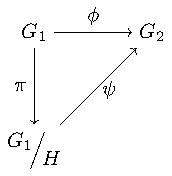
\includegraphics[width=0.35\linewidth]{Mathematics/2nd/Algebraic_structures/Images/theorem1.tex} 
    \captionof{figure}{}
    \label{theorem1}
\end{minipage}\par
In particular, if $H=\ker\phi$, then $\varphi$ is injective and therefore there is an isomorphism $\varphi:G_1/\ker\phi\rightarrow\im\phi$.
\end{theorem}
\begin{theorem}
Let 
\begin{align*}
    \phi:\mathbb{Z}&\longrightarrow\quot{\mathbb{Z}}{n\mathbb{Z}}\times\quot{\mathbb{Z}}{m\mathbb{Z}}\\
    1&\longmapsto(\Bar{1},\Bar{1})
\end{align*}
be a group morphism. Then, $\phi$ induces a morphism $\psi:\mathbb{Z}/nm\mathbb{Z}\rightarrow\mathbb{Z}/n\mathbb{Z}\times\mathbb{Z}/m\mathbb{Z}$. Moreover, $\psi$ is injective if and only if $\gcd(n,m)=1$ and in this case $\psi$ is an isomorphism. 
\end{theorem}
\begin{corollary}
Let $n,m\in\mathbb{Z}$ be two coprime integers and $a,b\in\mathbb{Z}$. The system of congruences $$\left\{\begin{array}{l}
    x\equiv a\mod{n}  \\
    x\equiv b\mod{m}  \\
\end{array}\right.$$ has solutions and these are of the form $x\equiv c\mod{nm}$, where $c\equiv a\mod{n}$ and $c\equiv b\mod{m}$.
\end{corollary}
\begin{definition}
Let $(G,\cdot)$ be a group and $(H,\cdot)$, $(K,\cdot)$ be subgroups of $(G,\cdot)$. We define the \textit{products of group subsets $K$, $H$} as the sets \begin{gather*}
    H\cdot K=\{h\cdot k:h\in H,k\in K\},\\
    K\cdot H=\{k\cdot h:k\in K,h\in H\}.
\end{gather*}
\end{definition}
\begin{prop}
Let $(G,\cdot)$ be a group and $(H,\cdot)$, $(K,\cdot)$ be subgroups of $(G,\cdot)$ such that $H\lhd G$. Then, $(H\cdot K,\cdot)$ is a subgroup of $(G,\cdot)$ and $H\cdot K=K\cdot H$.
\end{prop}
\begin{prop}
Let $(G,\cdot)$ be a group and $(H,\cdot)$, $(K,\cdot)$ be subgroups of $(G,\cdot)$ such that $H\cap K=\{e\}$. If $H,K\lhd G$, then the map 
\begin{align*}
    \phi:H\times K&\longrightarrow H\cdot K\\
    (h,k)&\longmapsto h\cdot k
\end{align*}
is an isomorphism. In particular, $\forall h\in H$ and $\forall k\in K$, $h\cdot k=k\cdot h$.
\end{prop}
\begin{theorem}[Second isomorphism theorem]
Let $(G,\cdot)$ be a group and $(H,\cdot)$, $(K,\cdot)$ be subgroups of $(G,\cdot)$ such that $H\lhd G$. Then $H\cap K\lhd K$ and $$\quot{K}{H\cap K}\cong\quot{H\cdot K}{H}.$$
\end{theorem}
\begin{corollary}
Let $(G,\cdot)$ be a group and $(H,\cdot)$, $(K,\cdot)$ be subgroups of $(G,\cdot)$ such that $H\lhd G$. Then, $$|H||K|=|H\cap K||H\cdot K|.$$
\end{corollary}
\begin{lemma}
Let $(G,\cdot)$ be a group and $(H,\cdot)$, $(K,\cdot)$ be subgroups of $(G,\cdot)$ such that $H\lhd G$ and $H\subseteq K$. Then $H\lhd K$, $(K/H,*)$ is a subgroup of $(G/H,*)$ and moreover $$\quot{K}{H}\lhd\quot{G}{H}\iff K\lhd G.$$
\end{lemma}
\begin{theorem}[Third isomorphism theorem]
Let $(G,\cdot)$ be a group and $(H,\cdot)$, $(K,\cdot)$ be subgroups of $(G,\cdot)$ such that $H,K\lhd G$ and $H\subseteq K$. Then $K/H\lhd G/H$ and $$\quot{\left(\quot{G}{H}\right)}{\left(\quot{K}{H}\right)}\cong\quot{G}{K}.$$
\end{theorem}
\subsubsection*{Group actions}
\begin{definition}
Let $X$ be a set and $(G,\cdot)$ be a group. A \textit{(left) group action} is a function 
\begin{align*}
    *:G\times X&\longrightarrow X\\
    (g,x)&\longmapsto g*x
\end{align*}
satisfying the following properties:
\begin{enumerate}
    \item $e*x=x$, $\forall x\in X$.
    \item $(g_1\cdot g_2)*x=g_1*(g_2*x)$, $\forall x\in X$ and $\forall g_1,g_2\in G$.
\end{enumerate}
A set $X$ together with an action $*$ of $(G,\cdot)$ is usually called a \textit{(left) $G$-set}.
\end{definition}
\begin{lemma}
Let $(G,\cdot)$ be a group and $X$ be a $G$-set. For all $g\in G$ the function
\begin{align*}
    \ell_g:X&\longrightarrow X\\
    x&\longmapsto g*x
\end{align*} is bijective an its inverse is $\ell_{g^{-1}}$.
\end{lemma}
\begin{definition}
Let $(G,\cdot)$ be a group and $X$ be a $G$-set. For all $x,y\in X$, we say $x\backsim y\iff\exists g\in G:y=g*x$.
\end{definition}
\begin{prop}
The relation $\backsim$ is an equivalence relation.
\end{prop}
\begin{definition}
Let $(G,\cdot)$ be a group and $X$ be a $G$-set. If $x\in X$, we define the \textit{orbit of $x$} as: $$\mathcal{O}_x=[x]_\backsim=\{g*x:g\in G\}.$$
\end{definition}
\begin{definition}
Let $(G,\cdot)$ be a group and $X$ be a $G$-set. For $x\in X$, we define the \textit{stabilizer of $(G,\cdot)$ with respect to $x$} as the set: $$G_x=\{g\in G:g*x=x\}.$$
\end{definition}
\begin{prop}
Let $(G,\cdot)$ be a group and $X$ be a $G$-set. For all $x\in X$, $(G_x,\cdot)$ is a subgroup of $(G,\cdot)$.
\end{prop}
\begin{theorem}[Orbit-stabilizer theorem]
Let $(G,\cdot)$ be a group, $X$ be a $G$-set and $x\in X$. The surjective map
\begin{align*}
    \phi:G&\longrightarrow \mathcal{O}_x\\
    g&\longmapsto g*x
\end{align*}
induces a bijective map $\Tilde{\phi}:\quot{G}{\!\!\approx}\;\rightarrow\mathcal{O}_x$, where $\approx$ is the equivalence relation $g_1\approx g_2\iff g_2^{-1}\cdot g_1\in G_x$ $\forall g_1,g_2\in G$\footnote{Note that the notation $\approx$ for the equivalence relation correspond with the one defined in definition \ref{AS_equiv}.}. In particular if $G$ is finite, $$|\mathcal{O}_x|=|[G:G_x]|.$$
\end{theorem}
\begin{corollary}[Orbits formula]
Let $(G,\cdot)$ be a finite group and $X$ be a finite $G$-set. If $x_1,\ldots,x_m$ are the elements of $X$ and $|\mathcal{O}_{x_i}|=1$ for $i=1,\ldots,r$, then:
\begin{equation}
    |X|=r+\sum_{i=r+1}^m|\mathcal{O}_{x_i}|=r+\sum_{i=r+1}^m|[G:G_{x_i}]|.
    \label{EA-obritsformula}
\end{equation}
\end{corollary}
\subsubsection*{Applications of orbits formula}
\begin{theorem}[Cauchy's theorem]
Let $(G,\cdot)$ be a finite group of order $n$ and $p$ be a prime number. If $p\mid n$, then $(G,\cdot)$ has an element of order $p$. 
\end{theorem}
\begin{corollary}
Let $p$ be an odd prime number. Then groups of order $2p$ are isomorphic to $(\mathbb{Z}/p\mathbb{Z},+)$ or $(D_{2p},\circ)$\footnote{$(D_{2p},\circ)$ is the dihedral group, that is, the group of symmetries of a regular polygon of $p$ sides, which includes rotations and reflections. Note that $|D_{2p}|=2p$.}.
\end{corollary}
\begin{prop}
Let $(G,\cdot)$ be a group. The map 
\begin{align*}
    G\times G&\longrightarrow G\\
    (g,x)&\longmapsto g\cdot x\cdot g^{-1}
\end{align*} is an action of $(G,\cdot)$ over itself. It is called the \textit{conjugation action}.
\end{prop}
\begin{definition}[Center of a group]
Let $(G,\cdot)$ be a group. We define the \textit{center of $(G,\cdot)$} as $$Z(G)=\{z\in G:z\cdot g=g\cdot z\;\forall g\in G\}\footnote{Note that, by orbits formula \eqref{EA-obritsformula}, if we consider the conjugation action we have: $$|G|=|Z(G)|+\sum_{|\mathcal{O}_x|>1}|\mathcal{O}_x|$$}.$$
\end{definition}
\begin{prop}
Let $p$ be a prime number and $(G,\cdot)$ be a finite group of order $p^n$ for some $n\geq 1$. Then, $|Z(G)|>1$.
\end{prop}
\begin{lemma}
Let $(G,\cdot)$ be a group and $(H,\cdot)$ be a subgroup of $(G,\cdot)$. Consider the application \begin{align*}
    H\times\quot{G}{\approx}&\longrightarrow \quot{G}{\approx}\\
    (h,g\cdot H)&\longmapsto(h\cdot g)\cdot H
\end{align*}
This application defines an action of the subgroup $(H,\cdot)$ over the set $\quot{G}{\!\!\approx}$.
\label{AS_action1}
\end{lemma}
\begin{definition}
Let $(G,\cdot)$ be a group and $(H,\cdot)$ be a subgroup of $(G,\cdot)$. The \textit{normalizer of $(H,\cdot)$ in $(G,\cdot)$} is $$N_G(H)=\{g\in G:g\cdot h\cdot g^{-1}\in H\;\forall h\in H\}.$$
\end{definition}
\begin{lemma}
Let $(G,\cdot)$ be a group and $(H,\cdot)$ be a subgroup of $(G,\cdot)$. $(N_G(H),\cdot)$ is a subgroup of $(G,\cdot)$ containing $H$ and, moreover, $H\lhd N_G(H)$.
\end{lemma}
\begin{corollary}
Let $(G,\cdot)$ be a finite group and $(H,\cdot)$ be a subgroup of $(G,\cdot)$. Then by orbits formula applied to action defined on \ref{AS_action1}, we have: $$[G:H]=[N_G(H):H]+\sum_{|\mathcal{O}_x|>1}|\mathcal{O}_x|.$$
\end{corollary}
\begin{prop}
Let $(G,\cdot)$ be a group of order $n\in\mathbb{N}$, $p$ be a prime number such that $p\mid n$ and $(H,\cdot)$ be a subgroup of $(G,\cdot)$ of order $p^i$, $i\geq 1$. Suppose $p\mid[G:H]$. Then $p\mid[N_G(H):H]$.
\end{prop}
\subsubsection*{Sylow's theorems}
\begin{corollary}
Let $(G,\cdot)$ be a group of order $n\in\mathbb{N}$, $p$ be a prime number and $(H,\cdot)$ be a subgroup of $(G,\cdot)$ such that $|H|=p^i$, $i\geq 0$. Suppose $p\mid[G:H]$. Then, there is a subgroup $(H',\cdot)$ of $(G,\cdot)$ such that $(H,\cdot)$ is a subgroup of $(H',\cdot)$ and $|H'|=p^{i+1}$. Moreover, $H\lhd H'$ and $H'/H\cong\mathbb{Z}/p\mathbb{Z}$.
\end{corollary}
\begin{theorem}[First Sylow theorem]
Let $(G,\cdot)$ be a finite group and $p$ be a prime number. Suppose $|G|=p^r m$, where $r\geq 0$ and $\gcd(p,m)=1$. Then, there is a subgroup $(K,\cdot)$ of $(G,\cdot)$ of order $p^r$. Moreover there is a chain of subgroups $(H_i,\cdot)$ satisfying: $$\{e\}=H_0\lhd H_1\lhd\cdots\lhd H_r=K,$$ such that $H_{i+1}/H_i\cong\mathbb{Z}/p\mathbb{Z}$ for $0\leq i<r$.
\end{theorem}
\begin{definition}
Let $p$ be a prime number. A group $(G,\cdot)$ is a \textit{$p$-group} if $|G|=p^r$, for some $r\in\mathbb{N}$.
\end{definition}
\begin{definition}
Let $p$ be a prime number and $(G,\cdot)$ be a group. A \textit{Sylow $p$-subgroup} is a $p$-subgroup of $(G,\cdot)$ of maximum order.
\end{definition}
\begin{definition}
Let $(G,\cdot)$ be a finite group. We say $(G,\cdot)$ is \textit{soluble} if there is a chain of subgroups $(H_i,\cdot)$ of $(G,\cdot)$ satisfying: $$\{e\}=H_0\lhd H_1\lhd\cdots\lhd H_r=K,$$ and such that the subgroups $(H_{i+1}/H_i,*)$ are cyclic, $0\leq i<r$. 
\end{definition}
\begin{theorem}[Second Sylow theorem]
Let $(G,\cdot)$ be a finite group and $p$ be a prime number. Suppose $|G|=p^r m$, where $r\geq 0$ and $\gcd(p,m)=1$. Let $(K,\cdot)$ be a Sylow $p$-subgroup of $(G,\cdot)$. Then, if $(H,\cdot)$ is a subgroup of $(G,\cdot)$ of order $p^i$, $\exists g\in G$ such that $g\cdot H\cdot g^{-1}\subseteq K$. In particular two different Sylow $p$-subgroups $(K_1,\cdot)$ and $(K_2,\cdot)$ are conjugate, that is, there exists an element $g\in G$ such that $g\cdot K_1\cdot g^{-1}=K_2$.
\end{theorem}
\begin{theorem}[Third Sylow theorem]
Let $(G,\cdot)$ be a finite group and $p$ be a prime number. Suppose $|G|=p^r m$, where $r\geq 0$ and $\gcd(p,m)=1$. Let $(K,\cdot)$ be a Sylow $p$-subgroup of $(G,\cdot)$ and $n_p$ be the number of different Sylow $p$-subgroups of $(G,\cdot)$. Then, $n_p=[G:N_G(K)]$. Therefore, $n_p\mid m$ and $n_p\equiv1\mod p$. 
\end{theorem}
\end{multicols}
\end{document}